%% Figure from MATH 556 notes, section 43 (Lecture 18). From the board sketch (Lecture 18).
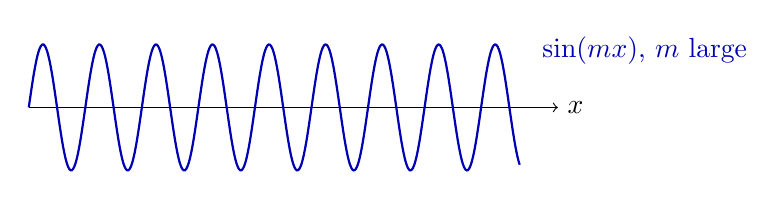
\begin{tikzpicture}[xscale=1.6, yscale=0.8]
    \draw[->] (0,0) -- (4.2,0) node[right] {$x$};
    \draw[thick, blue!70!black, domain=0:3.9, samples=400, smooth] plot (\x, {sin(14*\x r)});
    \node[blue!70!black, anchor=west] at (4.0,0.9) {$\sin(mx)$, $m$ large};
\end{tikzpicture}
